% Author: Izaak Neutelings (February 2021)
% https://mathworld.wolfram.com/PhasePortrait.html
\documentclass[border=3pt,tikz]{standalone}
\usepackage{amsmath} % for \dfrac
\usepackage{physics,siunitx}
\usepackage{tikz,pgfplots}
\usepackage{etoolbox} % ifthen
\usepackage[outline]{contour} % glow around text
\contourlength{1.1pt}
\usetikzlibrary{angles,quotes} % for pic (angle labels)
\usetikzlibrary{arrows.meta}
\usetikzlibrary{calc}
\usetikzlibrary{decorations.markings}
\usetikzlibrary{bending} % for arrow head angle
\tikzset{>=latex} % for LaTeX arrow head
\usepackage{xcolor}
\pgfplotsset{compat=newest}

\colorlet{xcol}{blue!60!black}
\colorlet{myred}{red!80!black}
\colorlet{myblue}{blue!80!black}
\colorlet{mygreen}{green!40!black}
\colorlet{mypurple}{red!50!blue!90!black!80}
\colorlet{mydarkred}{myred!80!black}
\colorlet{mydarkblue}{myblue!80!black}
\tikzstyle{xline}=[xcol,thick,smooth]
\tikzstyle{width}=[{Latex[length=5,width=3]}-{Latex[length=5,width=3]},thick]
\tikzstyle{mydashed}=[dash pattern=on 1.7pt off 1.7pt]
\tikzset{
  traj/.style 2 args={xline,postaction={decorate},decoration={markings,
    mark=at position #1 with {\arrow{<}},
    mark=at position #2 with {\arrow{<}}}
  }
}
\def\tick#1#2{\draw[thick] (#1)++(#2:0.12) --++ (#2-180:0.24)}
\def\N{100} % number of samples


\begin{document}


% PHASE DIAGRAM: Simple harmonic oscillator
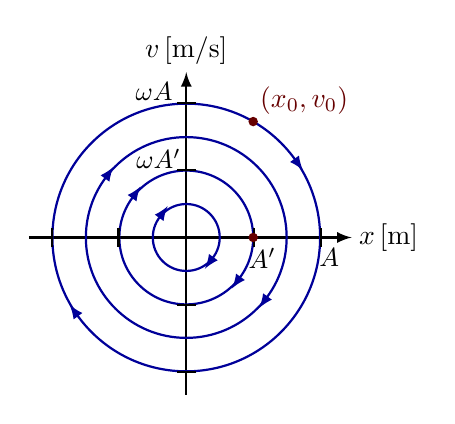
\begin{tikzpicture}
  \message{^^JPHASE DIAGRAM: Simple harmonic oscillator}
  \def\xmax{2.0}
  \def\A{1.7}
  \def\a{0.85}
  \def\ang{60}
  \coordinate (O) at (0,0);
  \coordinate (X) at (\A,0);
  \coordinate (R) at (\ang:\A);
  \coordinate (R') at (0:\a);
  \draw[->,thick] (-\xmax,0) -- (\xmax+0.1,0) node[right=-1] {$x$\,[m]};
  \draw[->,thick] (0,-\xmax) -- (0,\xmax+0.1) node[above=-1] {$v$\,[m/s]};
  \draw[traj={0.10}{0.60}] (0,0) circle(\A); % (\ang:\A) arc(\ang:\ang-360:\A);
  \draw[traj={0.40}{0.90}] (0,0) circle(\a);
  \draw[traj={0.40}{0.90}] (0,0) circle(0.75*\A);
  \draw[traj={0.40}{0.90}] (0,0) circle(0.25*\A);
  \tick{0,-\A-0.01}{0}; %node[left=-1,scale=1] {$A$};
  \tick{0, \A+0.01}{0} node[above=4,left=-2,scale=0.95] {$\omega A$};
  \tick{0,-\a-0.01}{0};
  \tick{0, \a+0.01}{0} node[above=4,left=-5,scale=0.95] {$\omega A'$};
  \tick{-\A-0.01,0}{90};
  \tick{-\a-0.01,0}{90};
  \tick{ \A+0.01,0}{90} node[right=3,below=-3,scale=0.95] {$A$};
  \tick{ \a+0.01,0}{90} node[right=3,below=-3,scale=0.95] {$A'$};
  \fill[myred!50!black] (R) circle (0.06) node[above right=-1] {$(x_0,v_0)$};
  \fill[myred!50!black] (R') circle (0.06); %node[below right=-2] {$(x_1,0)$};
  %\draw[->,mygreen!80!black] (\ang-15:1.1*\A) arc(\ang-15:\ang-40:0.9*\A);
  %\draw[->,mygreen!80!black] (-18:1.2*\a) arc(-18:-60:\a);
\end{tikzpicture}


% PHASE DIAGRAM - different parameters
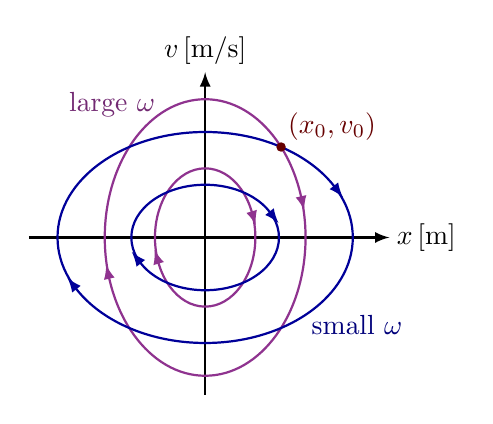
\begin{tikzpicture}
  \message{^^JPHASE DIAGRAM: different parameters}
  \def\xmax{2.0}
  \def\A{1.5}
  \def\ang{50}
  \def\ry#1{\A*sin(\ang)*sqrt(1/(1-(cos(\ang)/#1)^2))}
  %\def\rell#1{ {#1*\A} and {\A*sin(\ang)*sqrt(1/(1-(cos(\ang)/#1)^2))} }
  \coordinate (O) at (0,0);
  \coordinate (X) at (\A,0);
  \coordinate (R) at (\ang:\A);
  \draw[->,thick] (-1.12*\xmax,0) -- (1.12*\xmax+0.1,0) node[right=-1] {$x$\,[m]};
  \draw[->,thick] (0,-\xmax) -- (0,\xmax+0.1) node[above=-1] {$v$\,[m/s]};
  %\draw[xline] (0,0) circle(\A);
  \draw[traj={0.055}{0.555},mypurple]
    (0,0) ellipse({0.85*\A} and \ry{0.85});
  \draw[traj={0.07}{0.57},mypurple]
    (0,0) ellipse({0.5*0.85*\A} and 0.5*\ry{0.85});
  \draw[traj={0.07}{0.57}]
    (0,0) ellipse({1.25*\A} and \ry{1.25});
  \draw[traj={0.07}{0.57}]
    (0,0) ellipse({0.5*1.25*\A} and 0.5*\ry{1.25});
  \fill[myred!50!black] (R) circle (0.06) node[above right=-1] {$(x_0,v_0)$};
  %\draw[->,mygreen!80!black] (\ang-15:1.1*\A) arc(\ang-15:\ang-40:0.9*\A);
  \node[above left,mypurple!80!black] at (110:\A) {large $\omega$};
  \node[below right,xcol!80!black] at (-35:\A) {small $\omega$};
\end{tikzpicture}


% PHASE DIAGRAM - damped
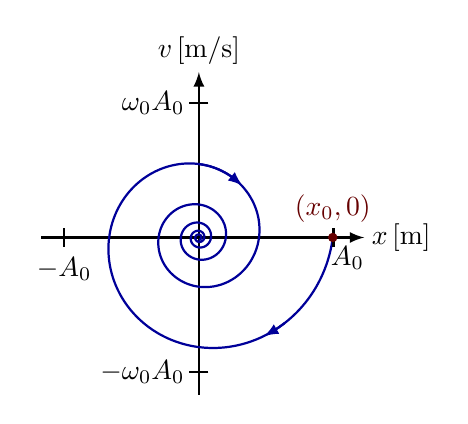
\begin{tikzpicture}
  \message{^^JPHASE DIAGRAM: damped}
  \def\xmax{2.0}
  \def\A{1.7}
  \def\a{0.8}
  \def\ang{60}
  \def\T{0.5}  % decay constant tau
  \def\om{2.5} % decay constant tau
  \coordinate (O) at (0,0);
  \coordinate (X) at (\A,0);
  \draw[->,thick] (-\xmax,0) -- (\xmax+0.1,0) node[right=-1] {$x$\,[m]};
  \draw[->,thick] (0,-\xmax) -- (0,\xmax+0.1) node[above=-1] {$v$\,[m/s]};
  \draw[->,xline,samples=100,variable=\t]
    plot[domain=0:0.06]({\A*exp(-\t/\T)*cos(360*\om*\t)},{-\A*exp(-\t/\T)*sin(360*\om*\t)})
    --++ (-150:0.08);
  \draw[->,xline,samples=100,variable=\t]
    plot[domain=0.05:0.34]({\A*exp(-\t/\T)*cos(360*\om*\t)},{-\A*exp(-\t/\T)*sin(360*\om*\t)})
    --++ (-40:0.08);
  \draw[xline,samples=200,variable=\t] %,line cap=round
    plot[domain=0.3:2.1]({\A*exp(-\t/\T)*cos(360*\om*\t)},{-\A*exp(-\t/\T)*sin(360*\om*\t)});
  \tick{0,-\A-0.01}{0} node[left=-2,scale=1] {$-\omega_0 A_0$};
  \tick{0, \A+0.01}{0} node[left=-2,scale=1] {$\omega_0 A_0$};
  \tick{-\A-0.01,0}{90} node[below=0,scale=1] {$-A_0$};
  \tick{ \A+0.01,0}{-90} node[right=5,below=3,scale=1] {$A_0$};
  \fill[myred!50!black] (X) circle (0.06) node[above=2] {$(x_0,0)$};
  %\draw[->,mygreen!80!black] (-20:1.05*\A) arc(-20:-55:0.6*\A);
\end{tikzpicture}


% PHASE DIAGRAM - pendulum
% Sources:
%   https://tex.stackexchange.com/questions/545590/phase-portrait-of-van-der-pol-oscillator-with-pgfplots
%   http://matlab.cheme.cmu.edu/2011/08/09/phase-portraits-of-a-system-of-odes/
% Instructions to compile this part of the code:
%   These curves were generated numerically with these MATLAB scripts:
%     https://github.com/IzaakWN/CodeSnippets/tree/master/LaTeX/TikZ/physics/dynamics_pendulum
%   To compile this part of the code, the curves need to be loaded via
%   external txt files. To download the txt files from GitHub, do e.g.
%     svn checkout https://github.com/IzaakWN/CodeSnippets/trunk/LaTeX/TikZ/physics/dynamics_pendulum/data ./dynamics_pendulum/data
\begin{tikzpicture}[scale=0.9]
  \message{^^JPHASE DIAGRAM: pendulum}
  \def\xmax{6.75}
  \def\ymax{3.15}
  \def\traj#1#2#3#4#5{ % pendulum trajectory curve
    \def\fname{dynamics_pendulum/data/pendulum_phase-#5.txt}
    \message{^^J Loading pendulum trajectory with initial omega = #5 from \fname...}
    \addplot[thin,xcol,postaction={decorate},decoration={markings,
             mark=at position #2 with {\arrow[thick,rotate=#4]{>}},
             mark=at position #3 with {\arrow[thick,rotate=#4]{>}}},#1]
      table {\fname};
    \addplot[xline,#1] table {\fname};
  }
  \def\pend#1#2{ % small pendulum diagram
    \def\R{0.55}
    \draw[mydarkblue,line width=0.9] ({(#1/180)*pi},-3.1) coordinate (O) --++ (#1-90:\R) coordinate(M);
    \draw[mydashed] (O) --++ (0,-0.9*\R) coordinate(B);
    \fill[mydarkblue!80!black] (O) circle(0.03);
    \draw[mydarkred,fill=myred] (M) circle(0.08);
    \ifnumcomp{#1}{>}{40}{
      \draw pic[-{>[flex'=1]},"$#2$"{scale=0.8},draw=black,angle radius=5,angle eccentricity=1.8] {angle = B--O--M};
    }{\ifnumcomp{#1}{<}{-40}{
      \draw pic[{<[flex'=1]}-,"$#2$"{scale=0.8},draw=black,angle radius=5,angle eccentricity=2.2] {angle = M--O--B};
    }{}}
  }
  \draw[->,thick] (-\xmax,0) -- (\xmax+0.1,0) node[right=-1] {$\theta$ [rad]};
  \draw[->,thick] (0,-\ymax) -- (0,\ymax+0.1) node[above=-2] {$\dot{\theta}$\,[rad/s]}; %\dfrac{\dd{\theta}}{\dd{t}}
  \begin{axis}[
      axis lines=none,anchor=origin,x=1cm,y=1cm,
      xmin=-2*pi,xmax=2*pi
    ]
    
    % CLOSED TRAJECTORIES
    \traj{}{0.150}{0.62}{9}{0p4}
    \traj{}{0.147}{0.61}{5}{0p8}
    \traj{}{0.145}{0.61}{2}{1p2}
    \traj{}{0.152}{0.64}{3}{1p6}
    \traj{myred}{0.130}{0.605}{0}{2p0}
    \begin{scope}[x filter/.code={\pgfmathparse{\pgfmathresult+2*pi}}]
      \traj{}{0.62}{0.81}{10}{0p4}
      \traj{}{0.61}{0.81}{5}{0p8}
      \traj{}{0.61}{0.82}{3}{1p2}
      \traj{}{0.64}{0.87}{0}{1p6}
      \traj{myred}{0.605}{0.858}{0}{2p0}
    \end{scope}
    \begin{scope}[x filter/.code={\pgfmathparse{\pgfmathresult-2*pi}}]
      \traj{}{0.150}{0.360}{10}{0p4}
      \traj{}{0.147}{0.360}{5}{0p8}
      \traj{}{0.145}{0.360}{3}{1p2}
      \traj{}{0.152}{0.382}{0}{1p6}
      \traj{myred}{0.130}{0.388}{0}{2p0}
    \end{scope}
    \draw[myred,very thick] (-pi-0.05,0) -- (-pi+0.05,0);
    \draw[myred,very thick] (pi-0.05,0) -- (pi+0.05,0);
    
    % OPEN TRAJECTORIES
    \traj{mypurple}{0.20}{0.80}{0}{2p4}
    \traj{mypurple}{0.20}{0.80}{0}{2p8}
    \begin{scope}[x filter/.code={\pgfmathparse{-\pgfmathresult}},
                  y filter/.code={\pgfmathparse{-\pgfmathresult}}]
      \traj{mypurple}{0.20}{0.80}{0}{2p4}
      \traj{mypurple}{0.20}{0.80}{0}{2p8}
    \end{scope}
    %\draw[->,thick] (-3*pi,0) -- (3*pi,0);
    
  \end{axis}
  \tick{-pi,0}{90} node[left=0.5,below=-4,scale=0.9] {\strut$-\pi$};
  \tick{ pi,0}{90} node[below=-4,scale=0.9] {\strut$\pi$};
  \tick{-2*pi,0}{90} node[left=4,below=-4,scale=0.9] {\strut\contour{white}{$-2\pi$}};
  \tick{ 2*pi,0}{90} node[right=1,below=-4,scale=0.9] {\strut\contour{white}{$2\pi$}};
  \tick{ 0, 2}{ 0} node[above=4.8,left=-6,scale=0.9] {$2\omega_0$};
  \tick{ 0,-2}{ 0} node[below=4.8,left=-6,scale=0.9] {$-2\omega_0$};
  \node[mydarkblue,scale=0.8,rotate=-57] at (1.92,0.69) {closed};
  \node[mydarkred,scale=0.8,rotate=-45] at (2.60,0.83) {separatrix};
  \node[mypurple,scale=0.8] at (3.1,2.20) {open};
  
  \pend{ 335}{}
  \pend{ 270}{}
  \pend{ 180}{\pi}
  \pend{  90}{} %\;\; \dfrac{\pi}{2}
  \pend{  25}{}
  \pend{ -25}{}
  \pend{ -90}{}
  \pend{-180}{-\pi}
  \pend{-270}{} %-\dfrac{\pi}{2}\;\;\;
  \pend{-335}{}
  
\end{tikzpicture}


\end{document}